\documentclass[10pt,aspectratio=169]{beamer}

\usepackage{presento/config/presento}
\usepackage{tikz}
\usetikzlibrary{shadings,shadows,calc,backgrounds,positioning}
\usepackage{tcolorbox}
\usepackage{adjustbox}
\tcbuselibrary{skins,breakable}
\usepackage[small, format=hang,justification=raggedright]{caption}

\usepackage[caption=false]{subfig}
%\usepackage{transparent}
\setbeameroption{show notes}

\usepackage[backend=bibtex]{biblatex}
\bibliography{bib/myrefs}

% figures
\usepackage {pgf}                                 % includepgf for bitmaps
\usepackage{graphicx}

% Information
\title{Extending Compiler Support for the BrainScaleS Plasticity Processor}
\subtitle{Bachelor's Thesis Presentation}
\author{Arthur Heimbrecht}
\institute{}
\date{\today}

\begin{document}


% Title page
{
\usebackgroundtemplate{
    \tikz[overlay, remember picture]\node[opacity=0.3, inner sep=0, outer sep=0, ] at (current page.center) {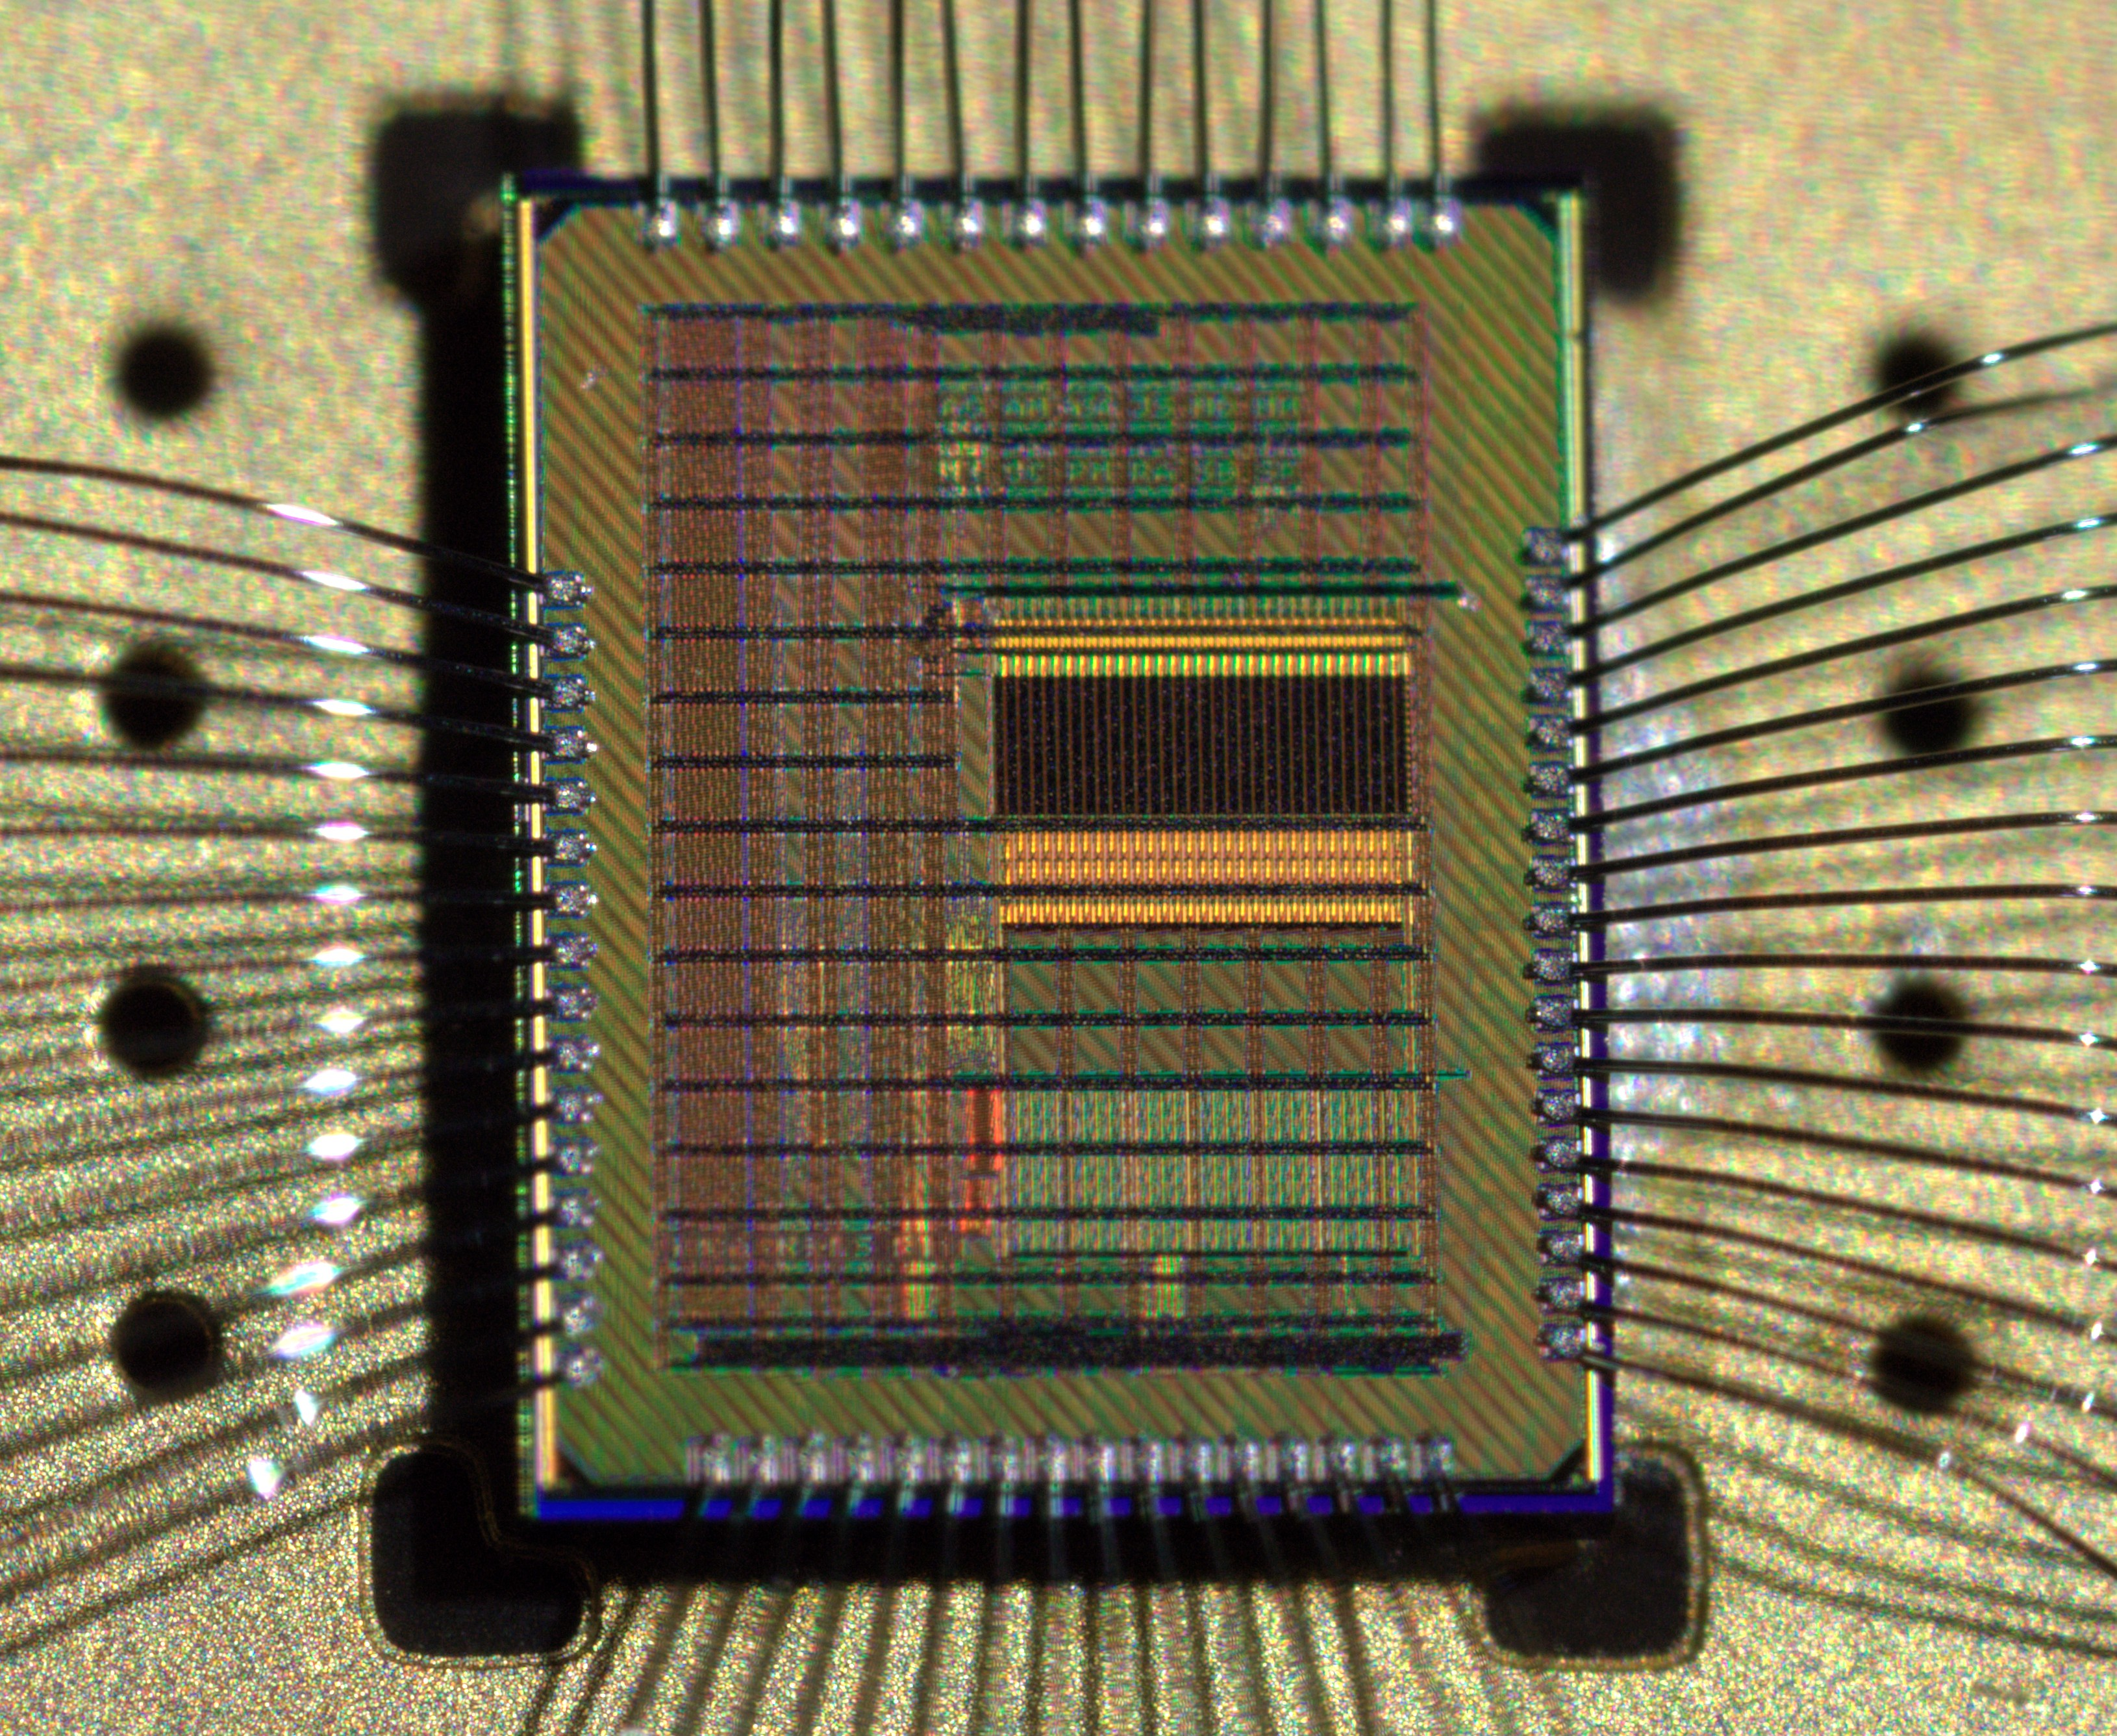
\includegraphics[width=\paperwidth]{pictures/dls_die_photo.jpg}};
}
\begin{frame}[plain]
\maketitle
\note{ Welcome everybody to this talk about my Bachelor thesis. As this is a quite technical talk, feel free to ask questions at any time.}
\note {The topic of my thesis was Extending Compiler Support for the BrainScaleS Plasticity Processor.}
\end{frame}

}

\begin{frame}{Contents}
\begin{columns}[c]
    \begin{column}{.5\textwidth}
        \begin{minipage}[t][0.5\textheight]{0.75\textwidth}
            \tableofcontents[sectionstyle=show, subsectionstyle=show/show/shaded]
        \end{minipage}\hfill
    \end{column}

    \begin{column}{.5\textwidth}
        \centering
        \begin{figure}
            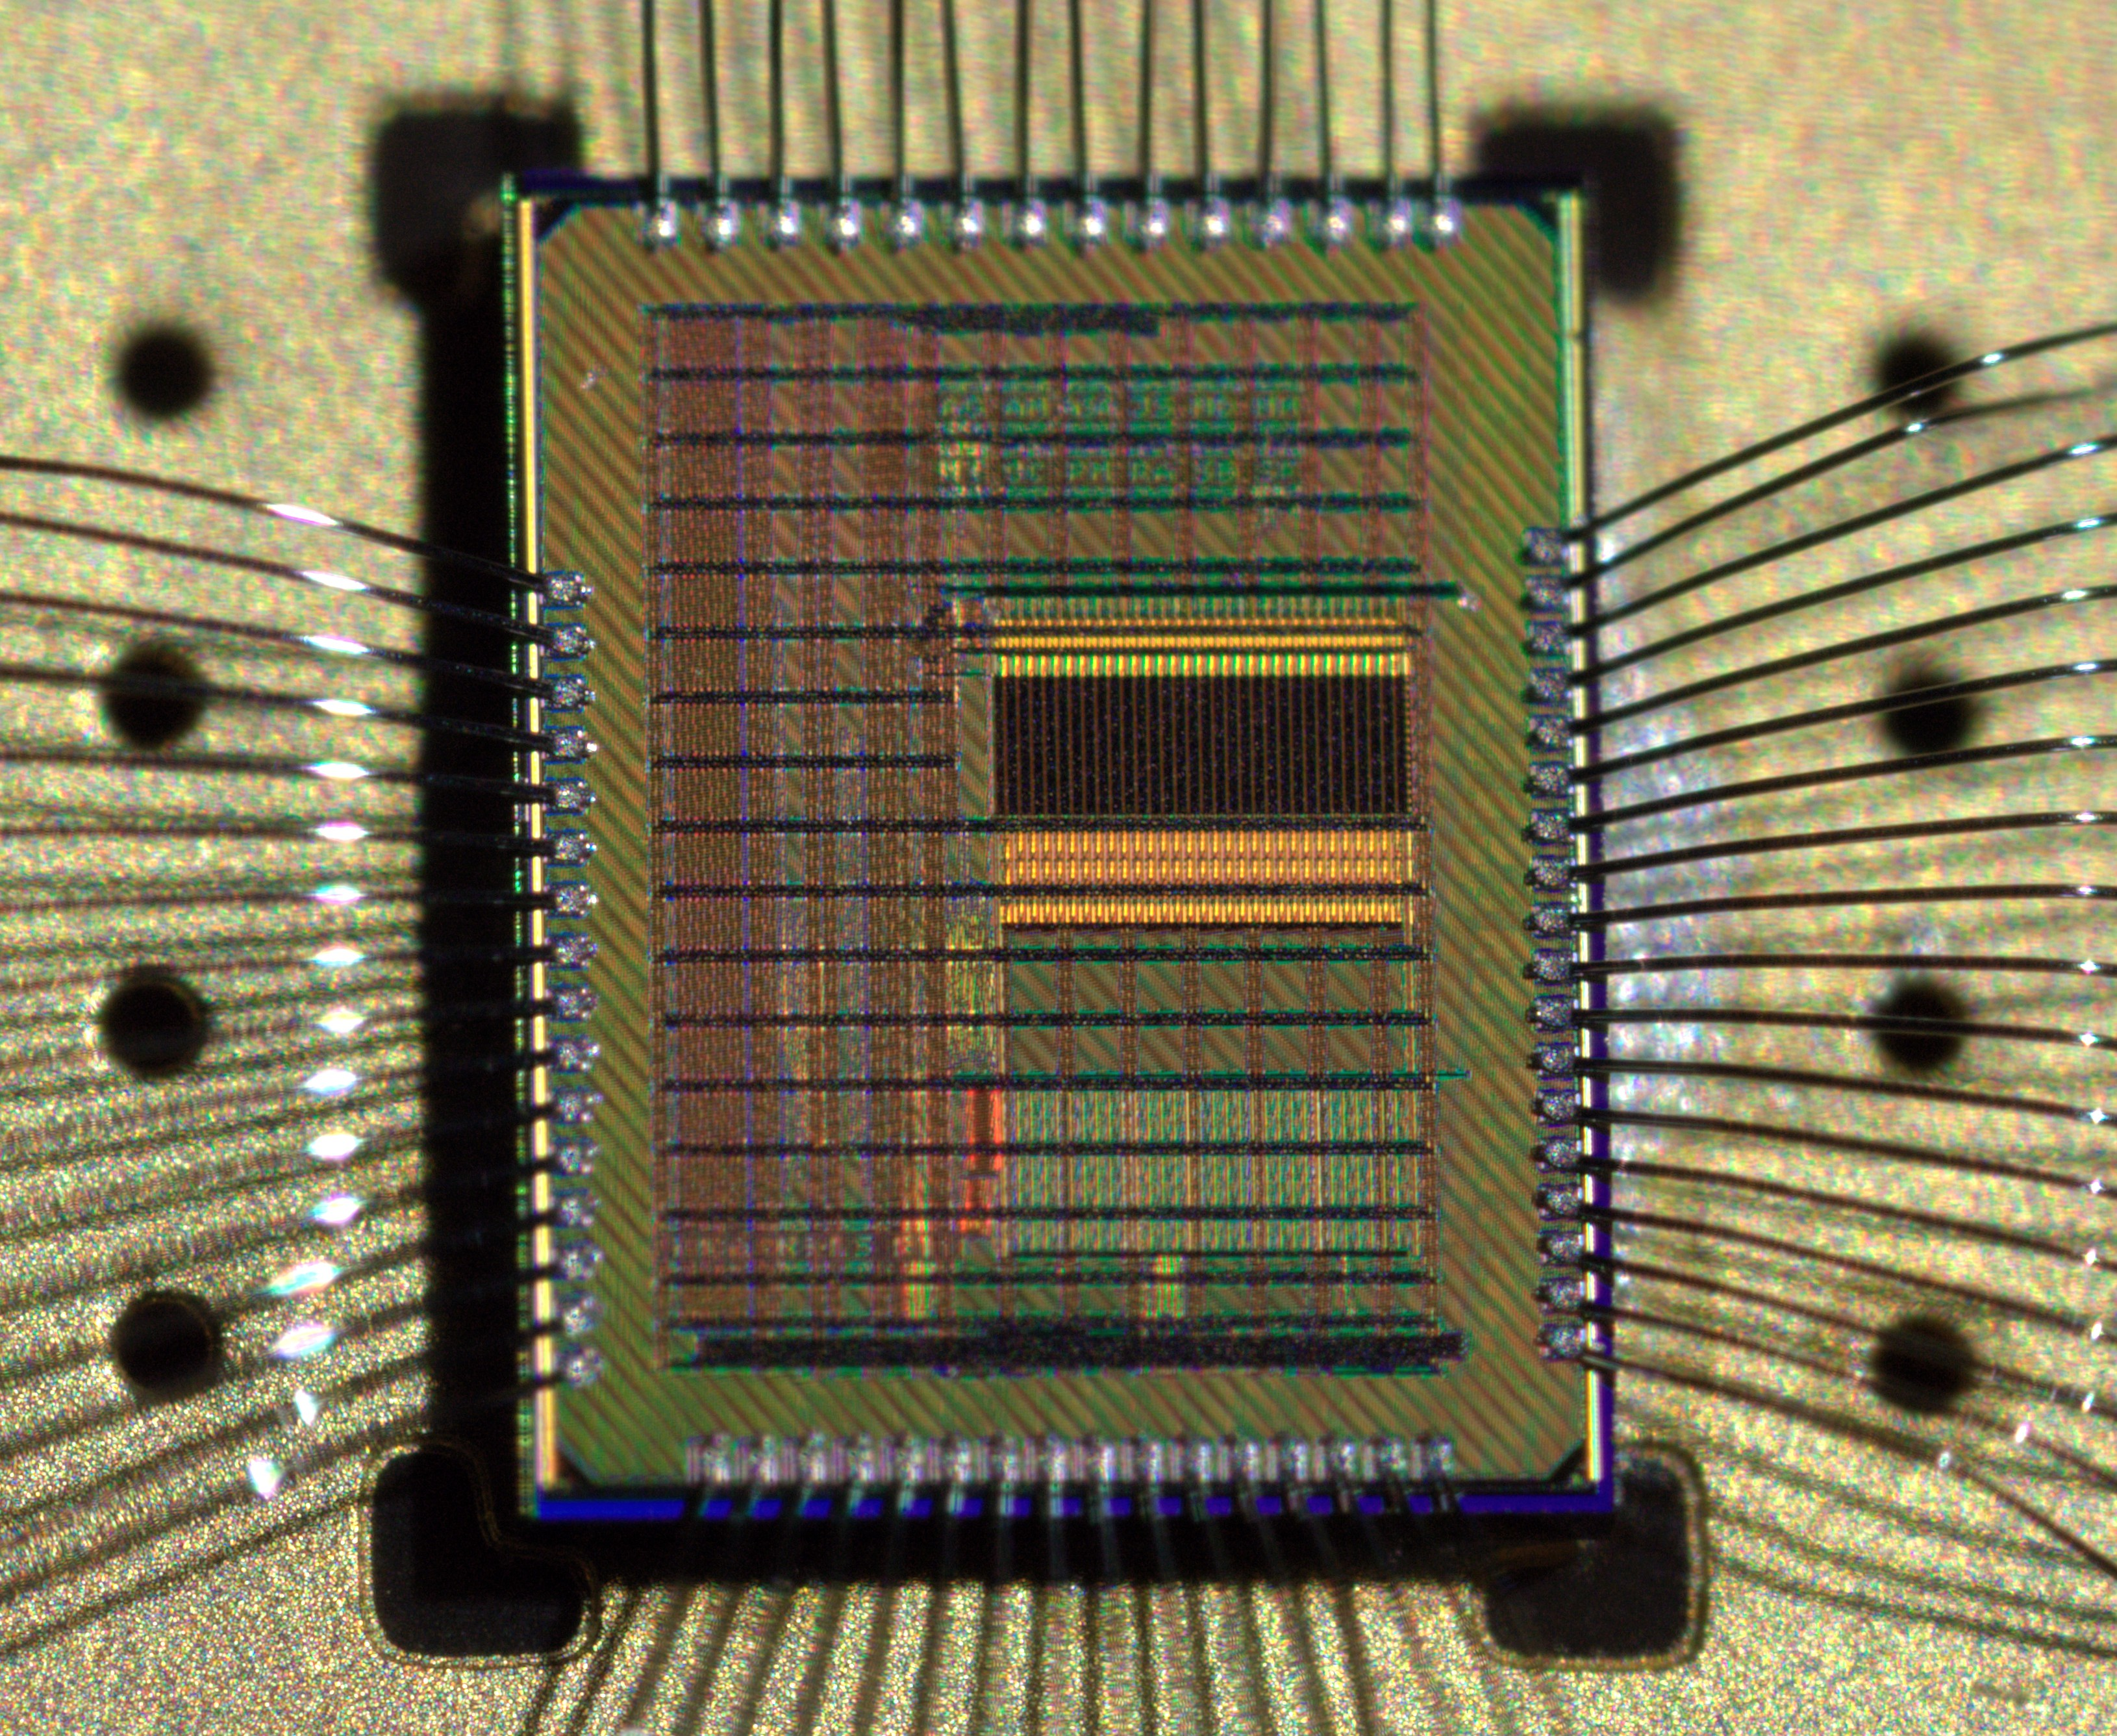
\includegraphics[width=\textwidth]{pictures/dls_die_photo.jpg}
            \caption{\label{fig:dls} Photograph of HICANN-DLS chip, \citeauthor{PPU}}
        \end{figure}
    \end{column}
\end{columns}
\note{
    as the title hints there are two main components to this talk, which are the plasticity processing unit (PPU) and Compilers.
    I will briefly talk about both of these and their applications.
    Afterwards I will explain, what I did during my thesis, which is of course followed by a short presentation of the results.

    But first I should explain, what the PPU is.
}
\end{frame}

% sections in the presentation
\section{PPU Architecture}
\begin{frame}{HICANN-DLS}
    \begin{columns}[c]
    \begin{column}{0.5\textwidth}
        \centering
        \begin{figure}
                \begin{adjustbox}{center, max width={.45\columnwidth}}
                    
\noindent{\begin{minipage}{\textwidth}
   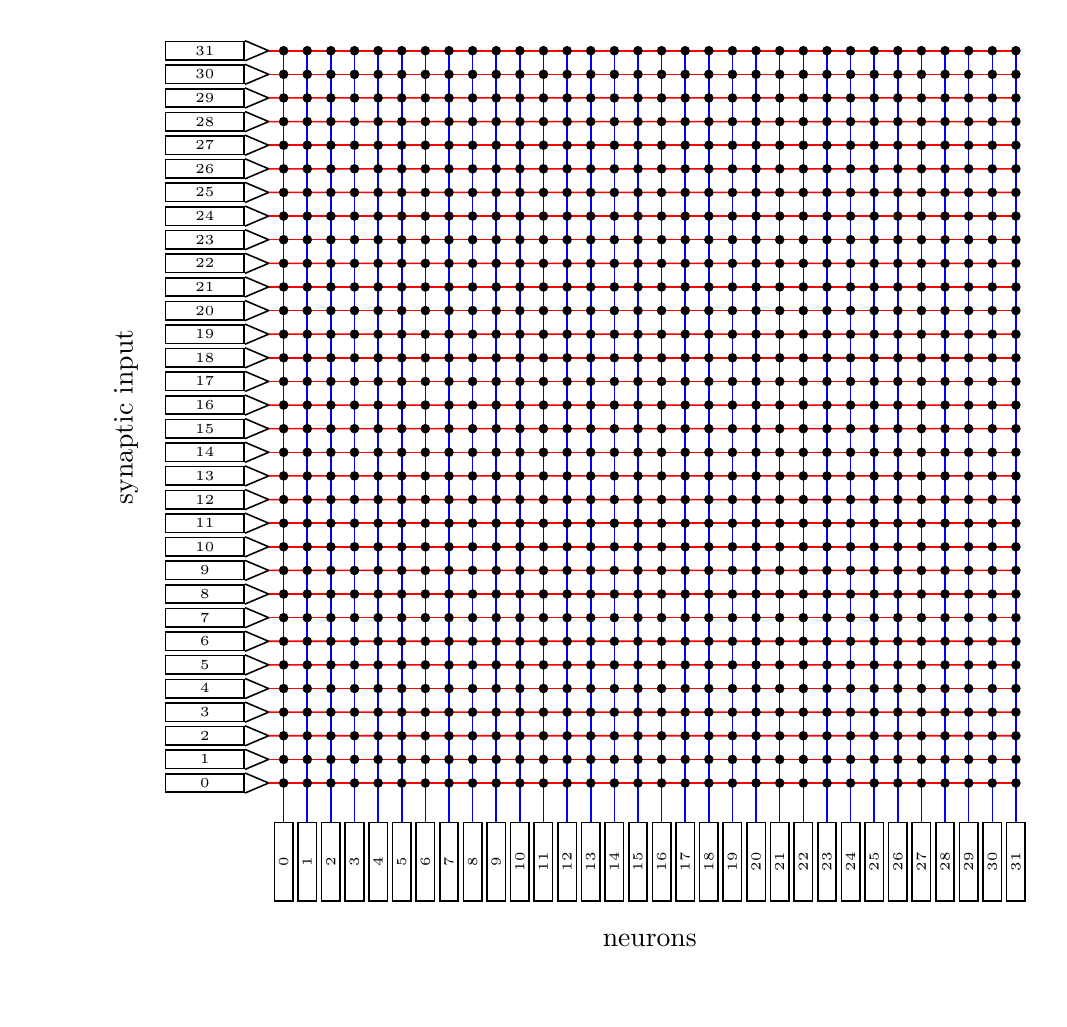
\begin{tikzpicture}[style={circle,draw,fill=black,minimum size=15}, line width=.2mm,
            vblock/.style={
            draw,
            fill=white,
            rectangle,
            minimum width=1.0cm,
            minimum height=0.3,
            font=\tiny},
            hblock/.style={
            draw,
            fill=white,
            rectangle,
            minimum width=.3,
            minimum height=1.0cm,
            font=\tiny}]

           \foreach \y in {0,...,31} 
           {
                      \node(domain)[vblock] (inrec\y) at (0, 0.3*\y + 1) {}; 
                      \draw[-] (inrec\y.north east) -- ($(inrec\y.north east)!.5!(inrec\y.south east)+(0.3,0)$) -- (inrec\y.south east);
                      \node (in\y) at (0, 0.3*\y + 1) {\tiny \y}; 
                      \draw[-, red] ($(inrec\y.north east)!.5!(inrec\y.south east)+(0.3,0)$) -- (0.3*31 + 1,0.3*\y + 1);
                  }
       \foreach \x in {0,...,31}
       { 
           \node(domain)[hblock] (neurec\x) at (0.3*\x + 1, 0) {}; 
           \node[rotate=90,] (neu\x) at (0.3*\x + 1, 0) {\tiny \x}; 
           \draw[-, blue] (neurec\x.north) -- (0.3*\x + 1,0.3*31 + 1);
           \foreach \y in {0,...,31} 
                  {\pgfmathtruncatemacro{\vlabel}{\y}
                  \draw [black,fill=black,radius=0.5mm, minimum size=0]  (0.3*\x + 1,0.3*\y + 1) circle;}
              }

              \node[rotate=90] (input) at (-1, 0.3*31/2 + 1) {synaptic input};
              \node[] (input) at (0.3*31/2 + 1, -1) {neurons};
   \end{tikzpicture}
\end{minipage}}

                \end{adjustbox}
            \caption{\label{fig:dls} Photograph of HICANN-DLS chip, modified from \citeauthor{PPU}}
        \end{figure}
    \end{column}

    \begin{column}{0.5\textwidth}
        \centering
        \begin{figure}
            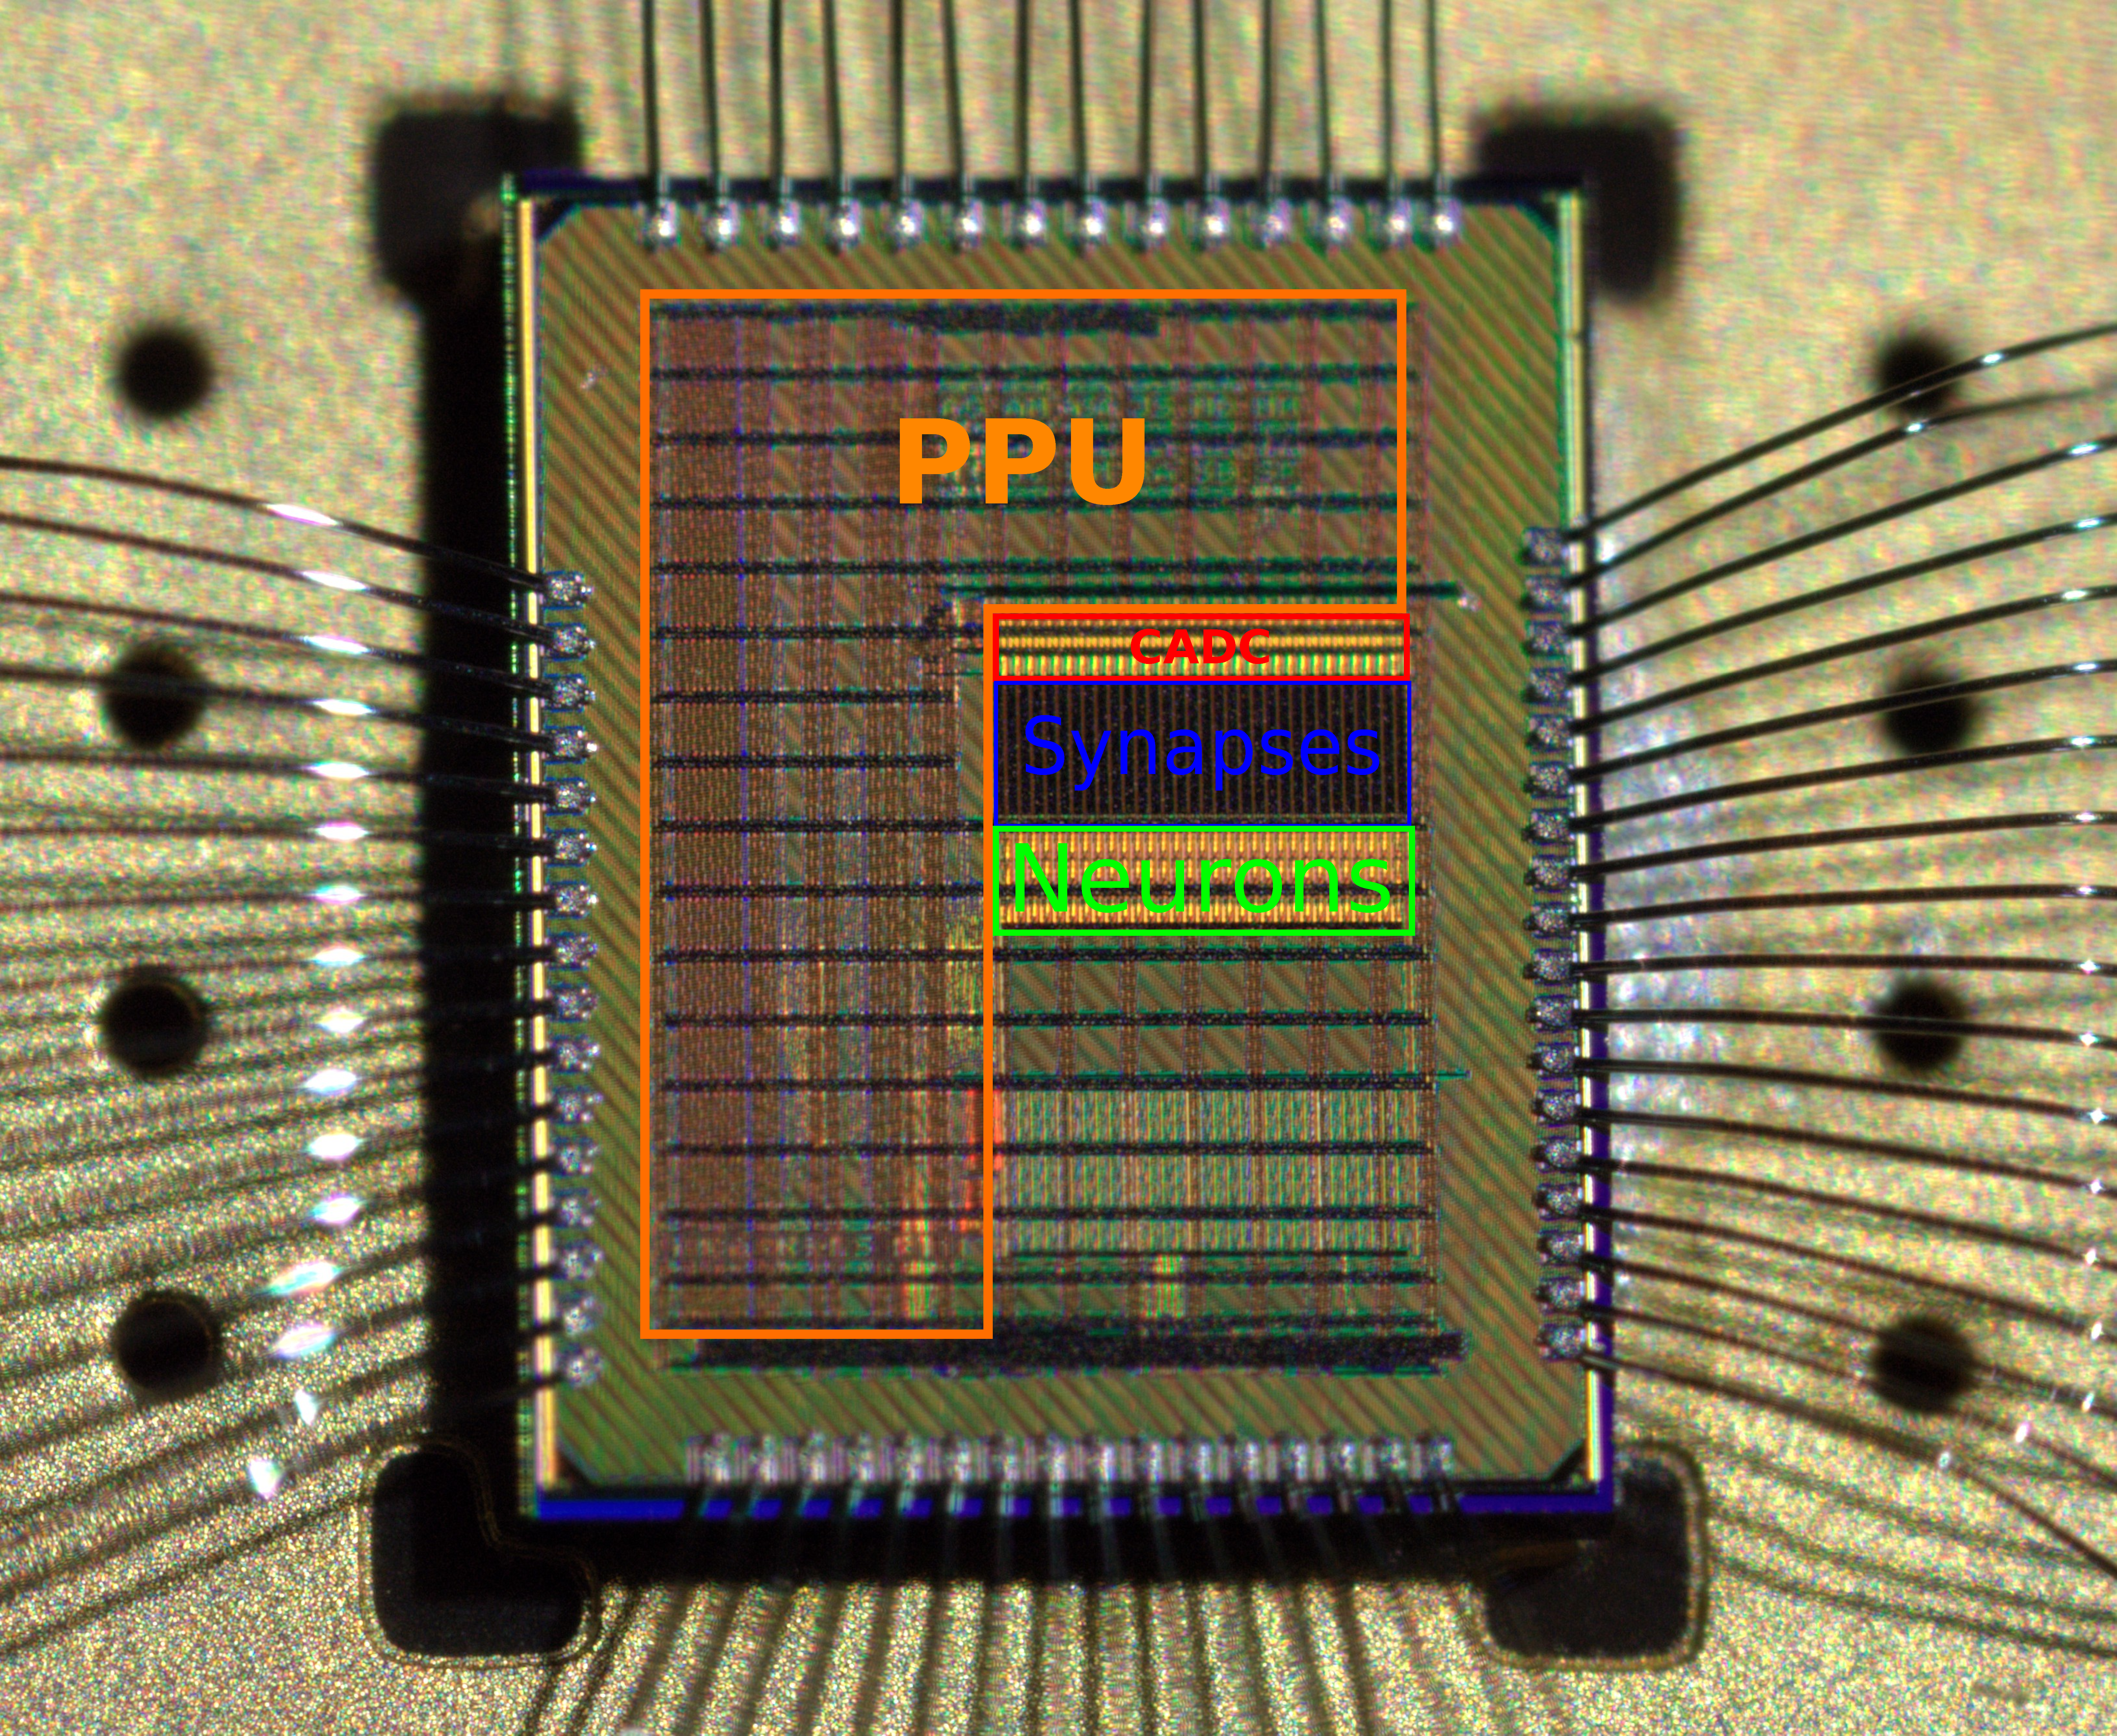
\includegraphics[width=\textwidth]{pictures/dls_marked.pdf}
            \caption{\label{fig:dls} Photograph of HICANN-DLS chip, modified from \citeauthor{PPU}}
        \end{figure}
    \end{column}
    \note{
        I am assuming that everybody here probably has heard about the HICANN-DLS.
        In short it is a chip that emulates neural networks through neurons and synapses that are implemented directly on the chip.
        What is special about the DLS, is the addition of a PPU to the HICANN.
        It is capable of performing simple computation and allows for on-line plasticity directly on the chip.

        As you can see to the right I have added a picture of the HICANN ship and marked the physical compartments.
        The PPU actually takes up a large space on the chip but before I am going to talk about the PPU, I will talk about the other parts briefly
        First we have the neurons.
        There are 32 neurons on the HICANN-DLS and each neuron is a circuit that receives some input signal which can cause the neurons to spike.
        These signals come from the so called synapse array.
        It connect 32 pre-synaptic inputs to all 32 neurons.
        This gives a total of 1024 synapses on each HICANN.
        
        Each synapse is realized through a circuit that takes the input signal and modifies it with a synpatic weight, that is saved in each synapse.
        There are also other properties to each synapse, but for this presentation it is enough to focus on the synaptic weights.
        Each synaptic weight is 6 bits wide, which is equivalent to numbers between 0 and 63 or a fixed-point number with an accuracy of $2^{-6}$.
        Normally data segments are 8 bits wide, which is a byte, and the  superfluous bits are used for calibration of the synapse.
        
        The pre-synaptic inputs are handled by an FPGA, that takes care of spike routing.
        
        But there is also a correlation analog digital converter, that receives also signals of synapses if the forward signals to neurons.
        Through the CADC one can read out correlation that can be used for plasticity.

        The PPU is this remaining large section of the HICANN chip.
		This mostly is an existing architecture, that is called POWER architecture, which was extended with a custom vector extension which we will call s2pp.

		In general it is good to keep this in mind during this talk:
		The processing unit in HICANN DLS is called the PPU, the architecture with the vector extension is called nux architecture and the vector extension will be called s2pp.
}
    \end{columns}

\end{frame}
\begin{frame}{Plasticity Processing Unit}
    \begin{columns}[c]
    \begin{column}{0.5\textwidth}
        \begin{itemize}
            \item The design is \underline{clean}
        \end{itemize}
    \end{column}

    \begin{column}{0.5\textwidth}
        \centering
        \vspace*{3em}
        \begin{figure}
                \begin{adjustbox}{center, max width={.7\columnwidth}}
                    \tcbset
{enhanced,colframe=blue!70!black,colback=white!50!blue,colupper=red!50!black,
fonttitle=\bfseries,center title, size=small}

\centering

%\begin{tcolorbox}[enhanced jigsaw, width=\linewidth, remember as=pp, opacityframe=0.0, opacityback=0.0, nobeforeafter]
\tcbset
{enhanced,colframe=blue!70!black,colback=white!50!blue,colupper=red!50!black,
fonttitle=\bfseries,nobeforeafter,center title, noparskip, size=small}

\begin{tikzpicture}[line width=1mm]
    
    \node[] (c) at (0,0) {
    \begin{tcolorbox}[width=.65\linewidth, enhanced jigsaw, remember as=cpu, size=normal]
        \centering
        Processor
    
        \begin{tcolorbox}[enhanced jigsaw, noparskip,opacityframe=0.3, opacityback=0.3, width=\linewidth, height=.7cm, size=small, remember as=cs]
        \centering
        Control Section
        \end{tcolorbox}
    
        \begin{tcolorbox}[enhanced jigsaw, noparskip,opacityframe=0.3, opacityback=0.3, width=\linewidth, size=small, fontupper=\footnotesize]
            \centering
    
            \begin{tcolorbox}[enhanced, width=\linewidth, remember as=alu]
                \centering
                ALU
            \end{tcolorbox}
            \begin{tcolorbox}[enhanced, width=\linewidth, remember as=rf]
                \centering
                Register File
            \end{tcolorbox}
    
            Operational Section
        \end{tcolorbox}
    
    \end{tcolorbox}
    };
    \end{tikzpicture}
    
\begin{tikzpicture}[overlay,remember picture,line width=0.5mm]
    
    \node[] (a) at ($(cs.west)!.0!(cs.north west)-(1.5,0)$) {
        \begin{tcolorbox}[enhanced jigsaw, opacityframe=0.3, opacityback=0.3, height=0.7cm, width=.15\linewidth, remember as=in, watermark text=Input, nobeforeafter]
        \end{tcolorbox}
    };
    
    \node[] (b) at ($(cs.east)!.0!(cs.north east)+(1.5,0)$) {
    \begin{tcolorbox}[enhanced jigsaw, opacityframe=0.3, opacityback=0.3, height=0.7cm, width=.15\linewidth, remember as=out, watermark text=Output, nobeforeafter]
    \end{tcolorbox}
    };
    
    \draw[->, shorten >=-1.0mm] (in.east) -- ($(cs.west)!.0!(cs.north west)$);
    \draw[->, shorten >=-1.0mm] ($(cs.east)!.0!(cs.north east)$) -- (out.west);

    \draw[->, shorten >=-1.0mm] ($(cs.west)!.5!(cs.south west)$) to [out=225, in=180] (alu.west);
    \draw[->, shorten >=-1.0mm] (alu.east) to [out=20, in=315] ($(cs.east)!.5!(cs.south east)$);
    
    \draw[->, shorten >=-1.0mm] ($(alu.south)!.5!(alu.south east)$) -- ($(rf.north)!.5!(rf.north east)$);
    \draw[->, shorten >=-1.0mm] ($(rf.north)!.5!(rf.north west)$) -- ($(alu.south)!.5!(alu.south west)$);
\end{tikzpicture}


% \begin{tikzpicture}[overlay,remember picture,line width=1mm]
%     \draw[->, shorten >=-1.5mm] ($(cp.north)+(0,1)$) -- (sc.north);
%     \draw[->, shorten >=-1.5mm] (sc.south) -- (ps.north);
%     \draw[->, shorten >=-1.5mm] (ps.south) -- (sa.north);
%     \draw[->, shorten >=-1.5mm] (sa.south) -- (sco.north);
%     \draw[-] (sco.south) -- (me.north);
%     \draw[->, shorten >=-1.5mm] (me.south) -- (cg.north);
%     \draw[->, shorten >=-1.5mm] (cg.south) -- (tco.north);
%     \draw[->] (tco.south) -- ($(cp.south)+(0,-1)$);
% \end{tikzpicture}
% \begin{tikzpicture}[overlay,remember picture,line width=1mm]
%     \draw[-, draw=blue!30!white,line width=.5mm, shorten >=.2cm,shorten <=.1cm] (cmp.north east) -- (cp.north west);
%     \draw[-, draw=blue!30!white,line width=.5mm, shorten >=.2cm,shorten <=.1cm] (cmp.south east) -- (cp.south west);
% \end{tikzpicture}

                \end{adjustbox}
            \caption{\label{fig:processor} Schematic of Processor in von-Neumann Architecture}
        \end{figure}
    \end{column}
    \end{columns}
\note{	But before I shall go into more detail, I have to talk about processors in general.
		As you may know, next to all computing nowadays is done by processors which are often described as CPUs.
		The processors are normally built according to the von-Neumann architecture, which combines programs and data in the same memory.
		The processor fetches instructions from the memory and analyzes them to decide what to do.
		Most instructions get passed to the ALU that performs any sort of computation in the processor.
		To do this, the ALU has access to so called registers.
		These registers can hold small amounts of data but offer a very low access time.
		The ALU uses these registers for computation and saves results there as well.
		Data is then written separately into memory or new values for registers are loaded from memory.
		This usually takes a significant amount of time longer than access to registers and thus, programs try to use registers as much as possible.

		Instead of the ALU, some instructions can be passed to other units that can perform special instructions.
		These units may also use different registers.

		This is the case for the PPU.
		It includes a special vector extension that includes vector registers as well.
		Using vector registers is favorable for operations that use have to be applied to multiple values and can be done in parallel.
		
		This is the strength of the PPU as is allows to compute weight updates of up to 16 synapses at the same time, which increases performance significantly. 
		Although it induces a problem because the vector unit uses special instructions that are unique to the nux architecture.

}

\end{frame}

\begin{frame}{PPU Architecture}
    \begin{columns}[c]
    \begin{column}{0.5\textwidth}
        \begin{itemize}
            \item \begin{center}\largetext{The design is \underline{clean}}\end{center}
            \item \begin{center}\largetext{The rules are \underline{simple}}\end{center}
            \item \begin{center}\largetext{The code is \underline{extensible}}\end{center}
        \end{itemize}
    \end{column}

    \begin{column}{0.5\textwidth}
        \centering
        \begin{figure}
            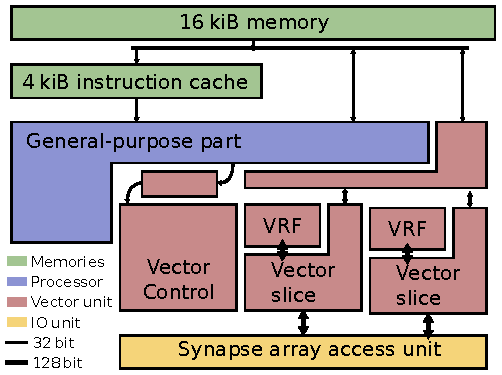
\includegraphics[width=.8\textwidth]{pictures/nux.pdf}
            \caption{\label{fig:nux} Structure of nux Architecture}
        \end{figure}
    \end{column}
    \end{columns}

\end{frame}



\section{GCC Structure}
\begin{frame}[fragile]{GCC Structure}
    \begin{columns}[c]
    \begin{column}{0.5\textwidth}
        \begin{itemize}
            \item \begin{center}\largetext{The design is \underline{clean}}\end{center}
            \item \begin{center}\largetext{The rules are \underline{simple}}\end{center}
            \item \begin{center}\largetext{The code is \underline{extensible}}\end{center}
        \end{itemize}
    \end{column}

    \begin{column}{0.5\textwidth}
        \centering
        \begin{figure}
            \begin{adjustbox}{center, max width={.5\columnwidth}}
                    \tcbset
    {my box/.style={enhanced,colframe=blue!70!black,colback=white!50!blue,colupper=red!50!black,
        fonttitle=\bfseries,nobeforeafter,center title, noparskip, size=small},
    every box on layer 1/.style={every box},
    every box on layer 2/.style={reset,my box}}
\begin{tcolorbox}[enhanced jigsaw, width=\textwidth, opacityframe=0.0, opacityback=0.0]
\begin{tcolorbox}[enhanced, height=.5cm, width=\linewidth, remember as=pp, opacityframe=0.0, opacityback=0.0]\end{tcolorbox}
\begin{tcolorbox}[enhanced, height=.7cm, width=\linewidth, watermark text=Preprocessor, remember as=pp]\end{tcolorbox}
\begin{tcolorbox}[tcbox raise base, width=\linewidth, enhanced jigsaw, remember as=cmp]
    \begin{tcolorbox}[enhanced, breakable, noparskip,opacityframe=0.3, opacityback=0.3, height=1.4cm, width=\linewidth, watermark text=Front-End, remember as=fe]
    \end{tcolorbox}
    \begin{tcolorbox}[enhanced, breakable, noparskip,opacityframe=0.3, opacityback=0.3, height=0.7cm, width=\linewidth, watermark text=Middle-End, remember as=me]
    \end{tcolorbox}
    \begin{tcolorbox}[enhanced, breakable, noparskip,opacityframe=0.3, opacityback=0.3, height=1.1cm, width=\linewidth, watermark text=Back-End, remember as=be]
    \end{tcolorbox}
\end{tcolorbox}

\end{tcolorbox}

\begin{tikzpicture}[overlay,remember picture,line width=1mm]
    \draw[->, shorten >=-1.5mm] ($(pp.north)+(0,1.5)$) -- node [left] {program code} (pp.north);
    \draw[->, shorten >=-1.5mm] (pp.south) -- (fe.north);
    \draw[->, shorten >=-1.5mm] (fe.south) -- (me.north);
    \draw[->, shorten >=-1.5mm] (me.south) -- (be.north);
    \draw[->] (be.south) -- node [left] {machine files} ++(0,-1.5);
\end{tikzpicture}

                    \tcbset
    {my box/.style={enhanced,colframe=blue!70!black,colback=white!50!blue,colupper=red!50!black,
        fonttitle=\bfseries,nobeforeafter,center title, noparskip, size=small},
    every box on layer 1/.style={every box},
    every box on layer 2/.style={reset,my box}}
\begin{tcolorbox}[enhanced jigsaw, width=\linewidth, remember as=pp, opacityframe=0.0, opacityback=0.0]
\begin{tcolorbox}[tcbox raise base, width=\linewidth, enhanced jigsaw, remember as=cp]
    \begin{tcolorbox}[enhanced jigsaw, breakable, noparskip,opacityframe=0.3, opacityback=0.3, width=\linewidth, size=small]
        \begin{tcolorbox}[enhanced,center title,width=\linewidth, remember as=sc, height=0.7cm,top=1mm,bottom=1mm]
            \begin{center}Scanner\end{center}
        \end{tcolorbox}
        \begin{tcolorbox}[enhanced,width=\linewidth, remember as=ps,top=1mm,bottom=1mm]
            \begin{center}Parser\end{center}  
        \end{tcolorbox}
        \begin{tcolorbox}[enhanced, width=\linewidth, remember as=sa,top=1mm,bottom=1mm]
            \begin{center}Semantic Analyzer \end{center} 
        \end{tcolorbox}
        \begin{tcolorbox}[enhanced, width=\linewidth, remember as=sco,top=1mm,bottom=1mm]
            \begin{center}Source Code Optimizer \end{center}
        \end{tcolorbox}
    \end{tcolorbox}
    \begin{tcolorbox}[enhanced jigsaw, breakable, noparskip,opacityframe=0.3, opacityback=0.3, height=0.7cm, width=\linewidth, remember as=me, watermark text=Middle-End]
    \end{tcolorbox}
    \begin{tcolorbox}[enhanced jigsaw, breakable, noparskip,opacityframe=0.3, opacityback=0.3, width=\linewidth, size=small]
        \begin{tcolorbox}[enhanced, width=\linewidth, remember as=cg,top=1mm,bottom=1mm]
            \begin{center}Code Generator  \end{center}
        \end{tcolorbox}
        \begin{tcolorbox}[enhanced, width=\linewidth, remember as=tco,top=1mm,bottom=1mm]
            \begin{center}Target Code Optimizer \end{center}
        \end{tcolorbox}
    \end{tcolorbox}
\end{tcolorbox}
\end{tcolorbox}
\begin{tikzpicture}[overlay,remember picture,line width=1mm]
    \draw[->, shorten >=-1.5mm] ($(cp.north)+(0,1)$) -- (sc.north);
    \draw[->, shorten >=-1.5mm] (sc.south) -- (ps.north);
    \draw[->, shorten >=-1.5mm] (ps.south) -- (sa.north);
    \draw[->, shorten >=-1.5mm] (sa.south) -- (sco.north);
    \draw[-] (sco.south) -- (me.north);
    \draw[->, shorten >=-1.5mm] (me.south) -- (cg.north);
    \draw[->, shorten >=-1.5mm] (cg.south) -- (tco.north);
    \draw[->] (tco.south) -- ($(cp.south)+(0,-1)$);
\end{tikzpicture}
\begin{tikzpicture}[overlay,remember picture,line width=1mm]
    \draw[-, draw=blue!30!white,line width=.5mm, shorten >=.2cm,shorten <=.1cm] (cmp.north east) -- (cp.north west);
    \draw[-, draw=blue!30!white,line width=.5mm, shorten >=.2cm,shorten <=.1cm] (cmp.south east) -- (cp.south west);
\end{tikzpicture}

            \end{adjustbox}
            \caption{\label{fig:compiler} Structure of Compiling Process and Compiler}
        \end{figure}
    \end{column}
    \end{columns}
\note{	This is of special significance when using a compiler.
		But why?
		I am quite sure that all of you have used compilers just recently and know what they do.
		And most will probably say that a compiler compiles code, or to be more specific it converts my program into a file that the computer can run.
		This is of course right and is follows the definition of a compiler, but there is much more to it.
		
		What we usually call compiler consists of sveral stages that follow diffeerent purposes and 
\end{frame}



\section{Extending GCC for the PPU}
\begin{frame}{Extending GCC for the PPU}
 \begin{center}
 \end{center}
\end{frame}

\section{Results}
\begin{frame}{Results}
 \begin{center}
 \end{center}
\end{frame}



\section{References}
\begin{frame}{References}
    \printbibliography
\end{frame}

\end{document}
